\documentclass[aspectratio=169]{beamer}
\usetheme[block=fill]{metropolis}
\usepackage{tikz}
\usetikzlibrary{shapes.geometric, arrows.meta, positioning, calc}

\title{Building a Reproducible Scholarly Search Toolkit}
\subtitle{Episode 24: Local File Providers \& Orchestration}
\author{Scholar Search Kit}
\date{}

\begin{document}

\begin{frame}[plain]
  \titlepage
\end{frame}

\begin{frame}{Episode Goal}
  \begin{alertblock}{The Goal}
    Create a \texttt{LocalFileProvider} to seamlessly inject local RIS files into the main orchestration pipeline.
  \end{alertblock}
  \vspace{0.5cm}
  The Orchestrator Engine doesn't care where data comes from. If we wrap our Importer in a Provider interface, the Engine will deduplicate local files automatically.
\end{frame}

\begin{frame}{The Hybrid Pipeline}
  \begin{center}
  \resizebox{0.7\linewidth}{!}{
  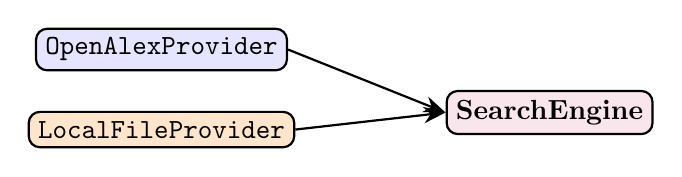
\begin{tikzpicture}[
      node distance=1cm and 2cm,
      api/.style={rectangle, draw, thick, rounded corners, minimum width=2.5cm, align=center, fill=blue!10},
      file/.style={rectangle, draw, thick, rounded corners, minimum width=2.5cm, align=center, fill=orange!20},
      eng/.style={rectangle, draw, thick, rounded corners, minimum width=2cm, align=center, fill=purple!10},
      arrow/.style={-{Stealth[scale=1.2]}, thick}
    ]
    
    \node[api] (a) {\texttt{OpenAlexProvider}};
    \node[file, below=0.5cm of a] (f) {\texttt{LocalFileProvider}};
    \node[eng, right=of a, yshift=-0.8cm] (e) {\textbf{SearchEngine}};
    
    \draw[arrow] (a.east) -- (e.west);
    \draw[arrow] (f.east) -- (e.west);
  \end{tikzpicture}
  }
  \end{center}
  \vspace{0.2cm}
  Multiple providers (APIs and Local Files) can feed into the same Engine simultaneously. The Deduplicator handles the overlap.
\end{frame}

\begin{frame}{Implementation: Query Handling}
  \begin{block}{Ignoring the Search String}
    The \texttt{SearchProvider} protocol requires a \texttt{Query} object.
  \end{block}
  
  \begin{itemize}
      \item A local file represents a search that was \textit{already} performed.
      \item We ignore the query \texttt{text} (so we don't accidentally drop valid Scopus results), but we DO enforce the \texttt{year\_min} and \texttt{year\_max} bounds.
      \item We attach the \texttt{query.id} to ensure provenance is tracked.
  \end{itemize}
\end{frame}

\begin{frame}{Verification}
  \begin{alertblock}{Success Criteria}
    \begin{itemize}
        \item Passing a \texttt{.ris} file to the Provider successfully yields matching documents.
        \item The Engine can ingest both a remote API result and a local file result and deduplicate them perfectly into one JSONL file.
    \end{itemize}
  \end{alertblock}
\end{frame}

\end{document}
